\begin{frame}{CART -- method summary}

\footnotesize

% \maketag{Supervised} 
\maketag{regression} \maketag{classification}
\maketag{Nonparametric} \maketag{White-box} \maketag{Feature selection}

\medskip

\begin{columns}[T, totalwidth=\textwidth]
\begin{column}{0.6\textwidth}
\highlight{General idea (CART -- Classification and Regression Trees)}
\begin{itemize}
  \item Start at root node containing all data
  \item Perform repeated \textbf{axis-parallel binary splits} in feature space to obtain
  \textbf{rectangular partitions} at terminal nodes $Q_1, \dots, Q_M$
  \item Splits based on reduction of node \textbf{impurity} \\
  $\rightarrow$ empirical risk minimization (\textbf{ERM})
  \item In each step:
  \begin{itemize}
    \item Find \textbf{optimal split} (feature-threshold combination) \\
    $\rightarrow$ greedy search
    \item Assign constant prediction $c_m$ to all obs. in $Q_m$\\
    $\rightarrow$ Regression: $c_m$ is average of $y$ \\
    $\rightarrow$ Classif.: $c_m$ is majority class (or class proportions)
    
  \item Stop when a pre-defined criterion is reached\\
  $\rightarrow$ See \highlight{Complexity control}
  \end{itemize}
  % \item Unless interrupted, splitting continues until each observation ends up 
  % in its own leaf node $\rightarrow$ \textbf{control complexity}
\end{itemize}

\end{column}
\begin{column}{0.45\textwidth}
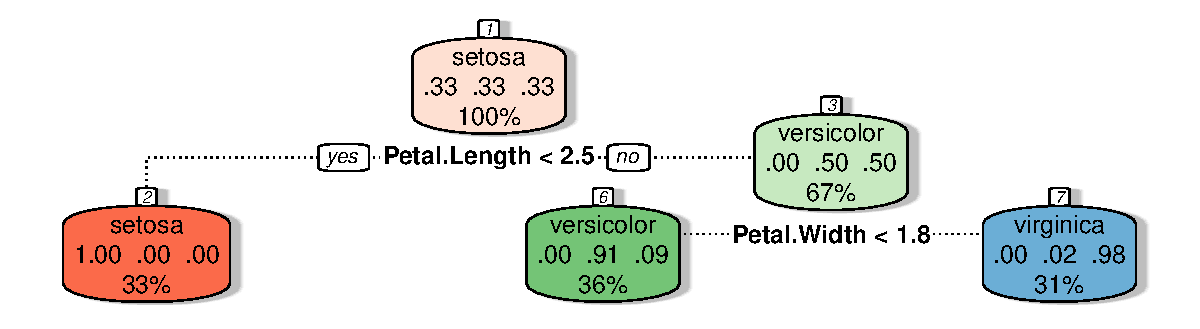
\includegraphics[width=\textwidth]{../slides/trees/figure/cart_treegrow_22}
\includegraphics[width=\textwidth]{   ../slides/trees/figure/cart_splitcriteria_1} 
\end{column}
\end{columns}

\medskip

%\medskip
    \highlight{Hypothesis space} ~~
$\Hspace = \left\{ \fx: \fx = \sum\limits_{m = 1}^M c_m \I(\xv \in Q_m) 
\right\}$


% \begin{minipage}[b]{0.5\textwidth}
%   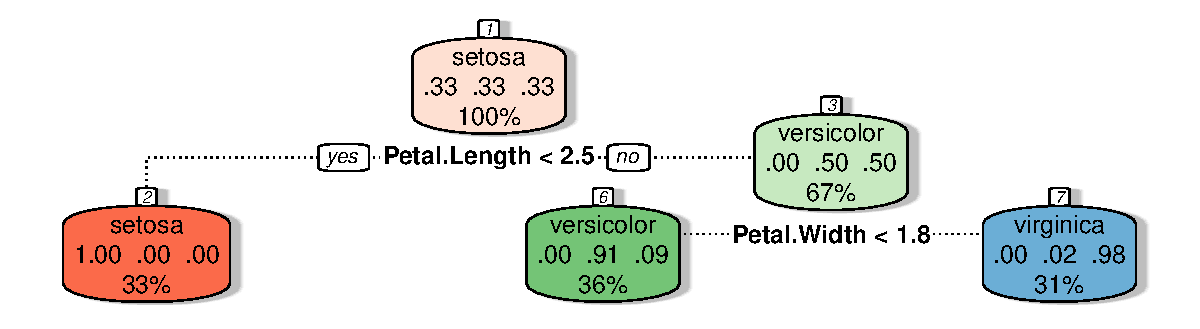
\includegraphics[width=\textwidth]{../slides/trees/figure/cart_treegrow_22} \\
%   \tiny{Classification tree for \texttt{iris} data after 3 splits}
% \end{minipage}
% \begin{minipage}[b]{0.49\textwidth}
%   \centering
%   \includegraphics[width=0.9\textwidth]{
%   ../slides/trees/figure/cart_splitcriteria_1} \\
%   \tiny{Corresponding prediction surface with axis-aligned boundaries}
% \end{minipage}%

\end{frame}

% ------------------------------------------------------------------------------

\begin{frame}{CART -- method summary}

\footnotesize

\begin{columns}[T, totalwidth=\linewidth]
    \begin{column}{0.6\linewidth}
    
\highlight{Empirical risk} \\
    \begin{itemize}
\item Splitting \textbf{feature $x_j$ at split point $t$} divides a parent node $\Np$ into two child nodes:
 \begin{align*}\Nl = \{ (\xv, y) \in \Np: x_j \leq t \} \text{ and } \Nr = \{ (\xv, y) \in \Np: x_j > t \}
      \end{align*}
  %\item Calculated after each split, i.e., at each node $\Np_t$ (which is not necessarily the terminal node $Q_t$)
  
\end{itemize}
    \end{column}
    \begin{column}{0.375\linewidth}
{\centering 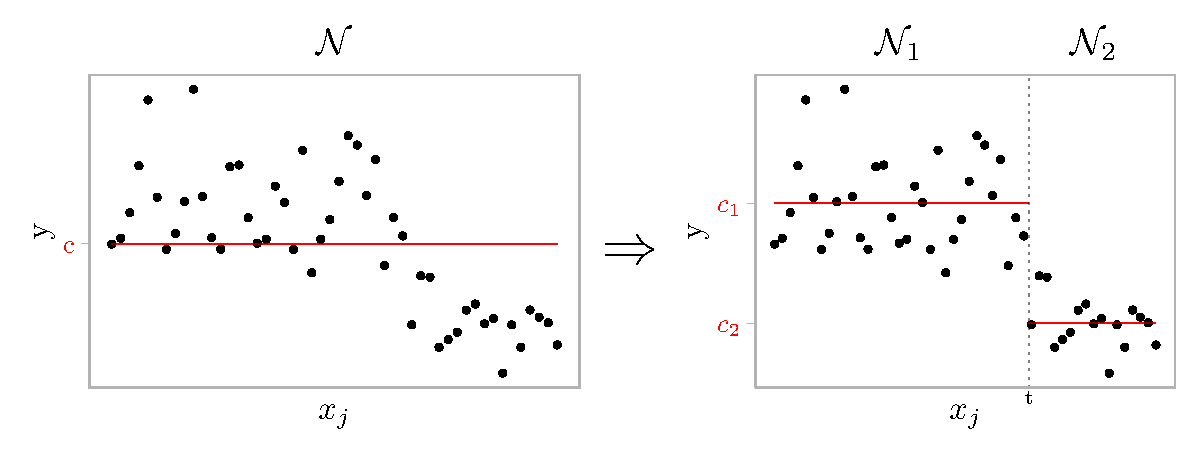
\includegraphics[width=0.975\textwidth]{../slides/trees/figure/cart_splitcriteria_2.pdf} 
}
\end{column}
\end{columns}
\begin{itemize}
  \item Compute empirical risks in child nodes and minimize their sum to find best split (impurity reduction):
     \begin{align*}
      \argmin_{j, t} \risk(\Np, j, t) &= \argmin_{j, t} \risk(\Nl) + \risk(\Nr) \;\;\; %\tfrac{|\Nr|}{|\Np|} 
      \end{align*}
      Note: If $\risk$ is the average instead of the sum of loss functions, we need to reweight: $\tfrac{|\Np_t|}{|\Np|} \risk(\Np_t)$
      
  \item In general, compatible with arbitrary losses -- typical choices:
  \begin{itemize}
    \footnotesize
    %\item $g$-way classification:
    %\begin{itemize}
      %\footnotesize
    %   \item $g$-way classification (\textbf{Brier score}): ~~
    %   $\risk(\Np) = \sum\limits_{(\xv,y) \in \Np} \sumkg
    %   \hat{\pik}^{(\Np)} (1 - \hat{\pik}^{(\Np)} )$
    %   % $\risk(\Np) = \sum\limits_{(\xv,y) \in \Np} \sumkg \left( \I(y = k)
    %   % - \pikx \right)^2$ 
    %   $\rightarrow$ \textbf{Gini} impurity
    %   \item $g$-way classification (\textbf{Bernoulli} loss): ~~
    %   $\risk(\Np) = \sum\limits_{(\xv,y) \in \Np} - \sumkg
    %   \hat{\pik}^{(\Np)} \log \hat{\pik}^{(\Np)}$
    %   % $\risk(\Np) = \sum\limits_{(\xv,y) \in \Np} \sumkg \I(y = k) \cdot
    %   % \log(\pikx)$ 
    %   $\rightarrow$ \textbf{entropy} impurity
    % %\end{itemize}

      \item $g$-way classification:
      \begin{tabular}{c |@{\vline}| c} 
 \textbf{Brier score} $\rightarrow$ \textbf{Gini} impurity & \textbf{Bernoulli} loss $\rightarrow$ \textbf{entropy} impurity \\ 
 \hline\\[-2ex]
 $\risk(\Np) = \sum\limits_{(\xv,y) \in \Np} \sum\limits_{k=1}^g
      \hat{\pik}^{(\Np)} (1 - \hat{\pik}^{(\Np)} )$ & $\risk(\Np) = -\sum\limits_{(\xv,y) \in \Np} \sum\limits_{k=1}^g
      \hat{\pik}^{(\Np)} \log \hat{\pik}^{(\Np)}$
\end{tabular}
      
    \item Regression (\textbf{quadratic} loss): ~~
    $\risk(\Np) = \sum\limits_{(\xv,y) \in \Np} (y - c)^2$ with $c = \frac{1}{|\Np|} \sum\limits_{(\xv,y) \in \Np} y$
  \end{itemize}
\end{itemize}

%\medskip

\highlight{Optimization}

\begin{itemize}
  \item \textbf{Exhaustive} search over all split candidates, choice of 
  risk-minimal split
  \item In practice: reduce number of split candidates (e.g., using quantiles instead of all observed values)
\end{itemize}

\medskip

% \highlight{Hyperparameters} ~~ \textbf{Complexity}, i.e., 
% number of terminal nodes $T$ (controlled indirectly, see \highlight{Implementation}) 

\end{frame}

% ------------------------------------------------------------------------------

\begin{frame}{CART -- Practical hints}

\footnotesize

\highlight{Hyperparameters and complexity control}

\begin{itemize}
%\item \textbf{Complexity} control affects number of terminal nodes using different parameters
  \item Unless interrupted, splitting continues until we have pure leaf nodes (costly + overfitting)
  \item Hyperparameters: Complexity (i.e., number of terminal nodes) controlled via tree depth, minimum number of observations per node, maximum number of leaves, minimum risk reduction per split, ...
  \item Limit tree growth / complexity via
  \begin{itemize}
    \item \textbf{Early stopping:} stop growth prematurely \\ $\rightarrow$ hard 
    to determine good stopping point before actually trying all combinations
    \item \textbf{Pruning:} grow deep trees and cut back in risk-optimal manner afterwards
  \end{itemize}
\end{itemize}

\medskip

% \highlight{Decision tree algorithms other than CART}
% %CART is a popular decision tree algorithm, 
% \begin{columns}[T, totalwidth=\linewidth]
%     \begin{column}{0.39\linewidth}
%     \vspace{-\parsep}
%         \begin{itemize}
% %\item AID (Sonquist and Morgan, 1964)
% \item CHAID (Kass, 1980)\\
% $\rightarrow$ Multi-way instead of binary splits
% \item C5.0 (Quinlan, 1993)
% \end{itemize}
%     \end{column}
%     \begin{column}{0.59\linewidth}
%     \vspace{-\parsep}
%         \begin{itemize}
% %\item Linear Model Trees (Potts, 2004)
% \item Unbiased Recursive Partitioning (Hothorn et al., 2006)\\
% $\rightarrow$ Conditional inference trees for unbiased splits
% \item Model-Based Recursive Partitioning (Hothorn et al., 2008)
% \end{itemize}
%     \end{column}
% \end{columns}
   
% \medskip

\highlight{Implementations}
\begin{itemize}
  \item \textbf{R:}
  \begin{itemize}
      \item \textbf{CART}: \texttt{mlr3} learners \texttt{LearnerClassifRpart} / 
    \texttt{LearnerRegrRpart}, calling \texttt{rpart::rpart()}
    \item \textbf{Conditional inference trees}: \texttt{partykit::ctree()}
    \item \textbf{Model-based recursive partitioning}: \texttt{partykit::mob()}
    \item \textbf{Rule-based models}: \texttt{Cubist::cubist()} for regression and \texttt{C50::C5.0()} for classification
  \end{itemize}
  \item \textbf{Python:} \texttt{DecisionTreeClassifier} / 
  \texttt{DecisionTreeRegressor} from package \texttt{scikit-learn}
\end{itemize}

\end{frame}
% ------------------------------------------------------------------------------

\begin{frame}{CART -- Pros \& Cons}

\highlight{Dual purpose of CART} ~~ 
% As CART is a highly \textbf{unstable} learner, it is used as a base learner in bagging (random forest) or boosting ensembles to reduce the variance and improve its performance.
\begin{itemize}
    \item \textbf{Exploration purpose} to obtain interpretable decision rules (here: performance/tuning is secondary)
    \item \textbf{Prediction model}: CART as base learner in \textbf{ensembles} (bagging, random forest, boosting) can improve stability and performance (if tuned properly), but becomes less interpretable
\end{itemize}

\medskip
\begin{columns}[onlytextwidth]
  \begin{column}{0.5\textwidth}
    \highlight{Advantages}
    \footnotesize
    \begin{itemize}
      \positem \textbf{Easy} to understand \& visualize (\textbf{interpretable})
      \positem Built-in \textbf{feature selection}\\
      $\rightarrow$ e.g., when features are not used for splitting
      \positem Applicable to \textbf{categorical} features \\
      $\rightarrow$ e.g., $2^m$ possible binary splits for $m$ categories\\
       $\rightarrow$ trick for regr. with L2-loss and binary classif.: categories can be sorted $\Rightarrow$ $m-1$ binary splits 
      \positem Handling of \textbf{missings} possible via surrogate splits
      \positem Models  \textbf{interactions}, 
      %effects between features 
      %naturally included, 
      even of higher order
      \positem \textbf{Fast} computation and good scalability
      \positem High \textbf{flexibility} with custom split criteria or leaf-node 
      prediction rules
      %\positem Used in \textbf{ensembles} (bagging, random forest, boosting), improves stability and performance
    \end{itemize}
  \end{column}
  \begin{column}{0.5\textwidth}
    \highlight{Disadvantages}
    \footnotesize
    \begin{itemize}
      \negitem Rather \textbf{poor generalization} %when used stand-alone 
      \negitem High \textbf{variance/instability}: model can change a lot when training data is minimally changed
      \negitem Can \textbf{overfit} if tree is grown too deep
      \negitem Not well-suited to model \textbf{linear} relationships
      \negitem \textbf{Bias} toward features with many unique values or categories
    \end{itemize}
  \end{column}
\end{columns}

\end{frame}

